%%%%%%%%%%%%%%%%%%%%%%%%%%%%%%%%%%%%%%%%%%%%%%%%%%%%%%%%%%%%%%%%%%%%%%%%%%%%%%%
% Document-Specific Settings
%%%%%%%%%%%%%%%%%%%%%%%%%%%%%%%%%%%%%%%%%%%%%%%%%%%%%%%%%%%%%%%%%%%%%%%%%%%%%%%

\documentclass[11pt]{article}

% include style package preamble
\usepackage{preamble}

% Babel dictionaries, include the languages we use in the paper
\usepackage[main=british]{babel}

% -----------------------------------------------------------------------------%
%   Relative pathnames for figures and tables                                  %
% -----------------------------------------------------------------------------%
\graphicspath{ {../../out/graphs/}{./figures/} } % figures path
\newcommand*{\TablesPath}{./tables/} % tables path
\newcommand*{\GraphsPath}{./graphs/}
% command for expanding table fragments
\makeatletter
\newcommand*\ExpandableInput[1]{\@@input#1 }
\makeatother

% High-Res Pictures Option
\DeclareGraphicsExtensions{.pdf, .png}

%----------------------------------------------------------------------------- %
%   External Appendix                                                          %
%----------------------------------------------------------------------------- %
% flag to attach the appendix at the end of the document
% set \stickappendixtrue if you want the appendix stick at the end of the
% document after the endfloats, otherwise \stickappendixfalse

\newif\ifstickappendix
\stickappendixfalse

% insert appendix file name
\newcommand{\AppendixName}{appendix.tex}

\usepackage{xr}
\ifx\me\usrtest
    \externaldocument{\AppendixName}
\else
    \overleafextdocument{\AppendixName}
\fi
\usepackage[toc,page]{appendix}

% ------------------------------------------------------------------------------
%   Data loader from .dat files
% ------------------------------------------------------------------------------
% Trick to import numbers from replication into the document and captions.
\usepackage{datatool}
\DTLsetseparator{;} % Set the separator between the columns.
% Loads mydata.dat with column headers 'thekey' and 'thevalue'
\DTLloaddb[noheader, keys={thekey,thevalue}]{scalars}{export_scalars.dat}
% Command to include the number in the text
\newcommand{\scalarinput}[1]{\DTLfetch{scalars}{thekey}{#1}{thevalue}}

% -----------------------------------------------------------------------------%
%   References path handler between overleaf projects and local                %
% -----------------------------------------------------------------------------%
% small snippet of code from stack overflow that allows me to assign the correct
% pathname for the references directory when using my local system instead of
% Overleaf when working with others. We also insert a quick hack for cross-
% referencing external documents in overleaf, otherwise the xr package breaks.
% https://tex.stackexchange.com/questions/107864/ifusername-foo-else-fi

\usepackage{catchfile}

% #1 = control sequence to define
% #2 = variable to get the value of
\newcommand{\getvar}[2]{%
    \CatchFileEdef#1{"|kpsewhich -var-value #2"}{\endlinechar=-1 }%
}

% specify your username locally
\def\me{dubidub}
\getvar{\usrtest}{USER}

\ifx\me\usrtest
    \newcommand*{\RefsPath}{../references}
\else
    \newcommand*{\RefsPath}{docs/references}
    \makeatletter
    \newcommand*{\addFileDependency}[1]{% argument=file name and extension
      \typeout{(#1)}
      \@addtofilelist{#1}
      \IfFileExists{#1}{}{\typeout{No file #1.}}
    }
    \makeatother
    
    \newcommand*{\overleafextdocument}[1]{%
        \externaldocument{#1}%
        \addFileDependency{#1.tex}%
        \addFileDependency{#1.aux}%
    }
\fi

%----------------------------------------------------------------------------- %
%   Working Paper Metadata                                                     %
%----------------------------------------------------------------------------- %

% Citation Aliases (if any)

% Dates
\usepackage[useregional]{datetime2}
% if I want to insert a specific date
\newcommand{\thedate}{\DTMdisplaydate{2017}{02}{21}{-1}}
\newcommand{\monthyeardate}{%
  \DTMenglishmonthname{\@dtm@month} \@dtm@year
}

% Here you can change the date presented in the paper title
% If I want a specific date I put in the date
% \date{This Version: \thedate}
% or if I want the date of today I just insert
\date{This Version: \today}
% or if I want just month and year
% \date{This Version: \monthyeardate}
% or I just remove it
%\date{}

\newcommand{\Acknowledgments}{
Acknowledgements with \lipsum[2]. Use footnote for providing further information about author (webpage, alternative address) \emph{and} funding agencies.
}

% main title
\title{Insert a Nice Title here with Title Case\thanks{\Acknowledgments}}
% optional subtitle, leave empty if you dont want it
\renewcommand{\subtitle}{An (optional) Nice Subtitle for the Paper}

\author{
    {David S.~Hippocampus}\thanks{Department of Computer Science, Pittsburgh, PA 15213, \texttt{hippo@cs.cranberry-lemon.edu}.} \\
    Department of Computer Science\\
    Cranberry-Lemon University\\
    %Pittsburgh, PA 15213 \\
    \texttt{hippo@cs.cranberry-lemon.edu} \\
    %% examples of more authors
    \And
    {Elias D.~Striatum}\thanks{Department of Electrical Engineering, Santa Narimana, Levand, \texttt{stariate@ee.mount-sheikh.edu}.} \\
    Department of Electrical Engineering\\
    Mount-Sheikh University\\
    %Santa Narimana, Levand \\
    \texttt{stariate@ee.mount-sheikh.edu} \\
    \AND
    {Elias D.~Striatum}\thanks{Department of Electrical Engineering, Santa Narimana, Levand, \texttt{stariate@ee.mount-sheikh.edu}.} \\
    Department of Electrical Engineering\\
    Mount-Sheikh University\\
    %Santa Narimana, Levand \\
    \texttt{stariate@ee.mount-sheikh.edu} \\
    \And
    {Elias D.~Striatum}\thanks{Department of Electrical Engineering, Santa Narimana, Levand, \texttt{stariate@ee.mount-sheikh.edu}.} \\
    Department of Electrical Engineering\\
    Mount-Sheikh University\\
    %Santa Narimana, Levand \\
    \texttt{stariate@ee.mount-sheikh.edu} \\
    %% \And
    %% Coauthor \\
    %% Affiliation \\
    %% Address \\
    %% \texttt{email} \\
}

%%% Add PDF metadata to help others organize their library
%%% Once the PDF is generated, you can check the metadata with
%%% $ pdfinfo template.pdf
\hypersetup{
    pdftitle={Insert a Nice Title here with Title Case},
    pdfsubject={q-bio.NC, q-bio.QM},
    pdfauthor={David S.~Hippocampus, Elias D.~Striatum},
    pdfkeywords={First keyword, Second keyword, More},
}

%%%%%%%%%%%%%%%%%%%%%%%%%%%%%%%%%%%%%%%%%%%%%%%%%%%%%%%%%%%%%%%%%%%%%%%%%%%%%%%
%   TITLE PAGE                                                                %
%%%%%%%%%%%%%%%%%%%%%%%%%%%%%%%%%%%%%%%%%%%%%%%%%%%%%%%%%%%%%%%%%%%%%%%%%%%%%%%

\begin{document}
\maketitle

\renewcommand{\thefootnote}{\arabic{footnote}}
\setcounter{footnote}{0}

%----------------------------------------------------------------------------- %
%   DRAFT DISCLAIMER                                                           %
%----------------------------------------------------------------------------- %

\draftdisclaimer

%----------------------------------------------------------------------------- %
%   ABSTRACT                                                                   %
%----------------------------------------------------------------------------- %

\noindent \lipsum[10]\\

%\vskip 0.8in
\vfill

{\noindent \textbf{JEL Classification:} P16; G21; D72; E51} \\
{\noindent \textbf{Keywords:} Monetary Policy, Income Inequality, Structural VAR, Average Propensity of Consume}\\

\newpage

%----------------------------------------------------------------------------- %
%  TABLE OF CONTENTS                                                           %
%----------------------------------------------------------------------------- %

% \tableofcontents
% \listoftodos

% \clearpage
% \newpage

%%%%%%%%%%%%%%%%%%%%%%%%%%%%%%%%%%%%%%%%%%%%%%%%%%%%%%%%%%%%%%%%%%%%%%%%%%%%%%%
%   DOCUMENT BODY                                                             %
%%%%%%%%%%%%%%%%%%%%%%%%%%%%%%%%%%%%%%%%%%%%%%%%%%%%%%%%%%%%%%%%%%%%%%%%%%%%%%%

\section{Section 1}

The finding in this paper cannot conclude the root cause of economic inequality in Cambodia. However, This study provides a broad overview and big picture to economists and policymakers to overlook and take ongoing action discussions and the way to design the innovation and creative policy for reducing economic inequality among households and individuals. According to the literature, many authors provide different perspectives associated with policy options to reduce economic inequality that can be resilient to technological change, globalization, and long-term economic development. \citet{Herran2005} suggest a higher level of democracy reduces the level of income inequality.\footnote{This is based on an empirical analysis covering 69 countries during the period from 1960 to 1996.} \citet{Bastagli2012, Breunig2019}; and \citet{Bastagli2012} suggest to increase graduation rates and improving education\footnote{For example, ''\textit{hybrid policies}`` like as the higher education contribution scheme (HECS) student loans with the collaboration between public and private sector \cite{Breunig2019}.}, well-designed labor market\footnote{A case of Brazil, \citet{Herran2005} suggest that provide effective training programs for the workforce will help them to highly competitive and high productivity.} and institutions policies\footnote{Especially, reducing the gap between employment protection on temporary and permanent work as well as a relatively high minimum wage that make people living better with the temporary inflation.}, foster the integration of immigrants, improving tax and transfer systems\footnote{Fiscal policy and cash transfer program are the primary indicator to reduce income inequality of low-income employees and poor households.}, promoting and considering to create the personal income tax system and boosting GDP per capita. An econometric test by \citet{GIZ2015} confirms that the reduction of inequality is possible even under open economy conditions if a given set of appropriate macroeconomic, labor, fiscal and social policies is adopted by governments.\footnote{\citet{GIZ2015} discusses the income inequality changes which have taken place in some representative developing regions during the 1980s--1990s, while inequality rose in the majority of the countries of these regions.}

Here I am testing the scalar input command: \textbf{the first beta is \scalarinput{first.value.beta}!}

\lipsum[3]

\input{\TablesPath table_3.tex}

\lipsum[4-5] \\

\improvement[inline]{Todo.}

\section{Section 2}

\subsection{Some Citations}

This is an example of section with citations by \citet{McAfee1992-sn} \citep[see][for citation in brackets]{McAfee1992-sn}. \lipsum

%-------------------------------------------------------------------------------
\begin{figure}[H]
  \caption{The growth of the broad money and inflation during 2010Q1--2021Q2}
  \label{fig:2}
  \begin{subfigure}[b]{0.5\linewidth}
    \caption*{Panel A: Broad Money} \vspace{-.5em}
    \label{fig:2a}
    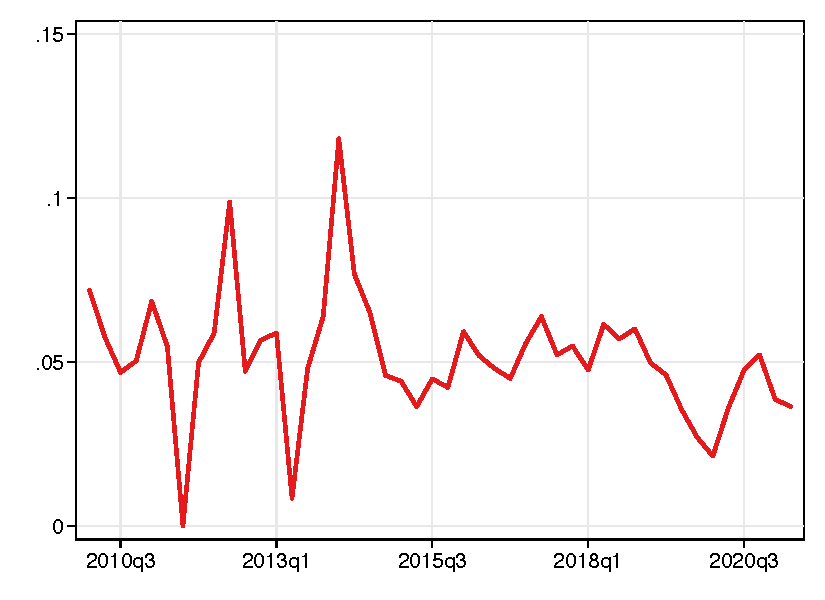
\includegraphics[width=1\linewidth]{moving_m2}
  \end{subfigure}%
  \hfil
  \begin{subfigure}[b]{0.5\linewidth}
    \caption*{Panel B: Inflation} \vspace{-.5em}
    \label{fig:2b}
    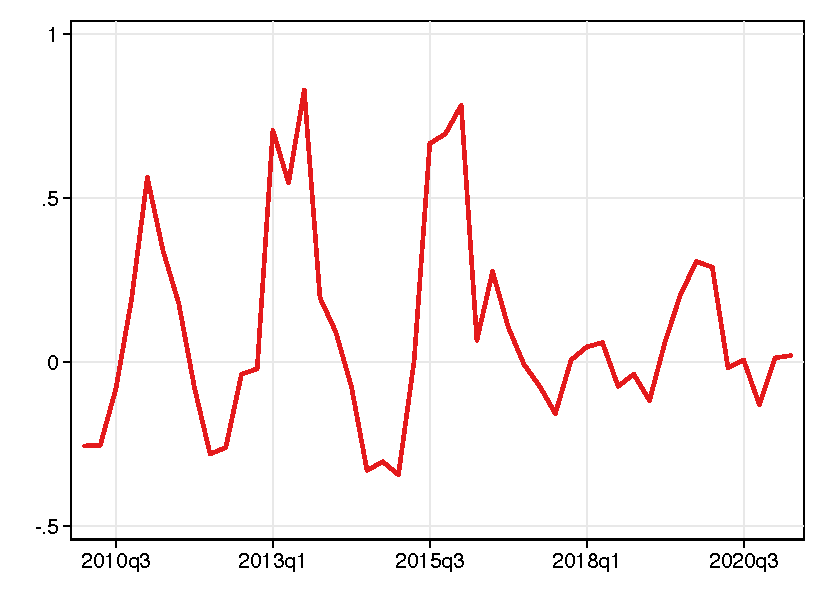
\includegraphics[width=1\linewidth]{moving_inflation}
  \end{subfigure}
  \begin{tablenotes}
    \footnotesize
    \item \textbf{Notes:} This two figures represent the moving average of the broad money and inflation between 2010Q1--2021Q2. Panel A reports the broad money and Panel B reports inflation rate growth. The $y$-axis reports the percentage change with multiply by 100 bias, the $x$-axis is the time period in quarters. The data uses to plot these figure come the National Bank of Cambodia and the National Institute of Statistics.
  \end{tablenotes}

\end{figure}

Table \ref{tab:gvar} summarizes the Granger-causality results for the six-variable VAR. It shows the $p$-values associated with the chi-squared statistic for testing whether the relevant sets of coefficients are zero. For example, if inflation does not help predict broad money, then the coefficient on the lags of inflation will all be zero in the reduced-form broad money supply equation. Inflation does not helps predict the broad money ($M2$), the unemployment rate, the exchange rate and the interest rate levels of statistical significance. Nevertheless, inflation helps predict output at the 10\% significance level with the $p$-value 0.076 or 7.6\%. My Granger tests show the $M2$ significantly impacts output, inflation and exchange rates at 1\% and 5\% of statistical significance (the $p$-value is 0.004, 0.017, and 0.036, respectively). In addition, the results reflect that the use of exchange rates as an instrument policy to control money supply in the market has a true consensus effect on other macroeconomic variables. As we see in Table \ref{tab:gvar}, the exchange rate has Granger-cause broad money and output statistically significant at a 1\% and 5\% level with $p$-value is 0.001 or 1\% and 0.097 or 9.7\%. Surprisingly, the unemployment rate has a consequence to many economic variables like inflation at a 1\% of statisitical significance, to $M2$ (4.9\%), the interest rate (4\%), and exchange rates at $p$-value 0.019 or 1.9\%.

%----------------------------------------------------------------------------- %
%   REFERENCES                                                                 %
%----------------------------------------------------------------------------- %

\clearpage\newpage
\bibliographystyle{aea}
%\bibliography{\RefsPath/references,\RefsPath/otherreferences}
\bibliography{references}
% \printbibliography
\clearpage

% include appendix if wanted
\ifstickappendix
  \processdelayedfloats
  \includepdf[pages=-]{\AppendixName}
\fi

%----------------------------------------------------------------------------- %
%   END DOCUMENT                                                               %
%----------------------------------------------------------------------------- %

\end{document}
